\section{Introduction}

\IEEEPARstart{F}{ollowing} a planned trajectory on a robot while
compensating execution errors has been extensively studied in the 90's
for mobile robots \cite{91icra.samson,
  98deLucaOrioloSamson}. Surprisingly, this issue has not been
explicitely addressed in the literature concerning navigation for
legged robots, although these machines are also prone to execution
errors while moving.

One way of indirectly tackling the problem consists of regularly
replanning the motion of the robot from its current configuration to
the goal. This strategy enables the robot to be reactive to
environment changes as well as to execution
errors~\cite{05humanoids.michel,
  06icra.MichelChestnut,10springer.chestnut}. On the other hand, it
requires short planning time and induces heavy CPU load. It might even
not be always be possible. Indeed most fast replanning schemes rely on
a simplified model~\cite{01icra.KajitaKanehiro} of the robot
neglecting momenta generated by the leg motions. These assumptions are
not met for small robots like Nao~\cite{wikipedia.nao} with a large
ratio of mass distributed in the legs and with a small CPU.

Moreover, to produce a really feasible movement, additional
constraints must be satisfied: no auto-collision should occur during
the movement for instance.


\begin{figure}[ht!]
  \begin{center}
    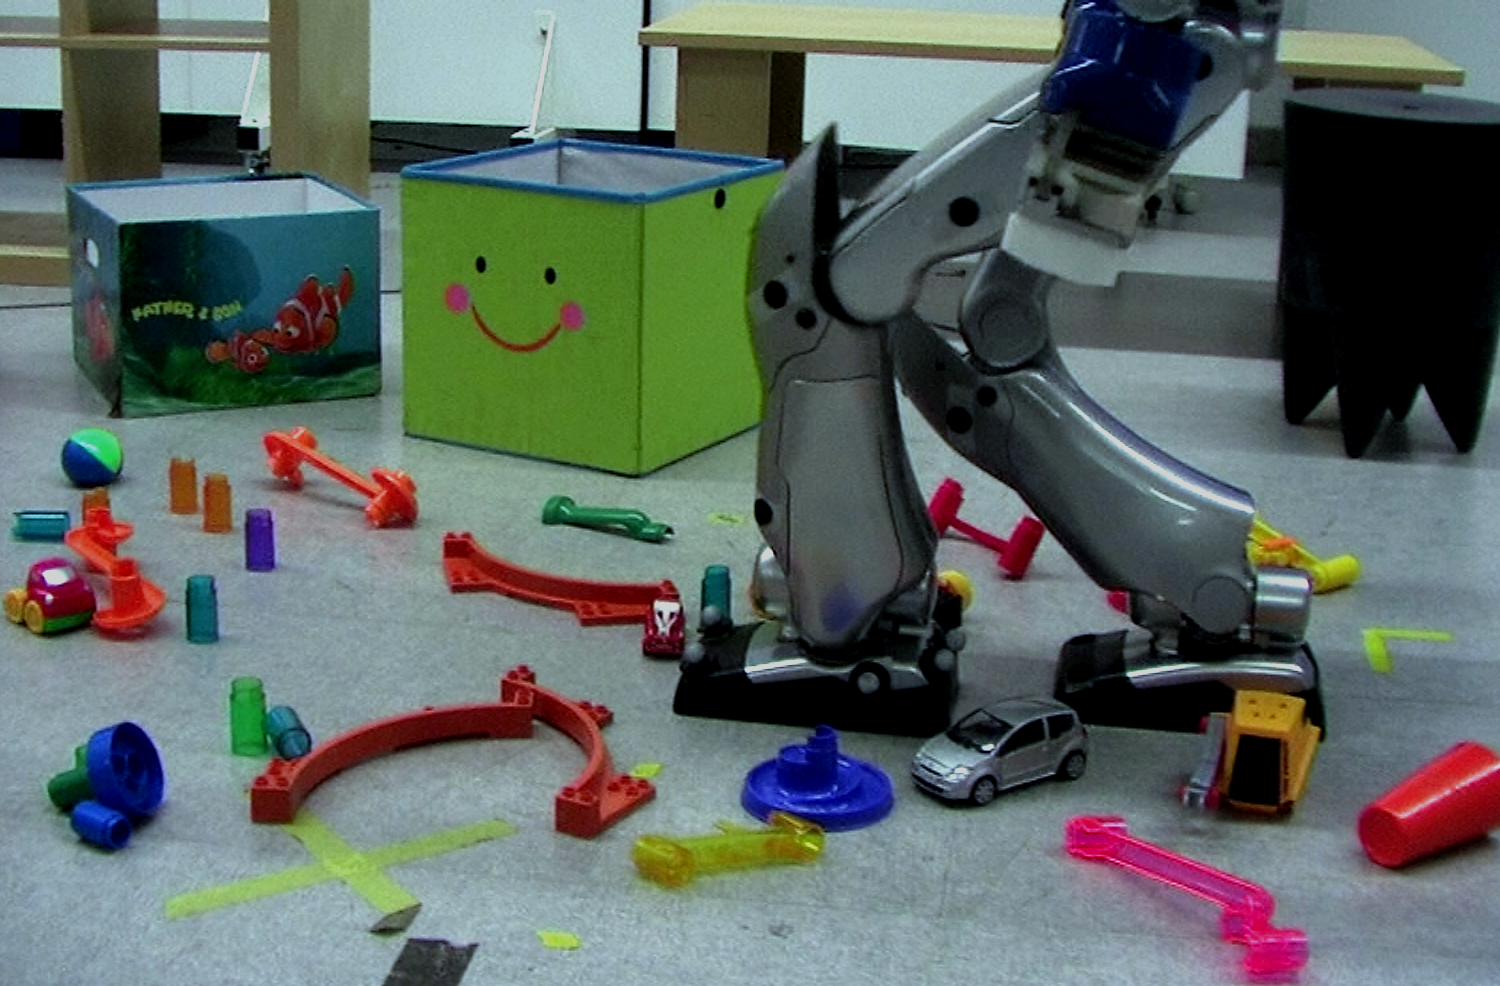
\includegraphics[width=.45\textwidth]{fig/exp.png}
  \end{center}
% 4cm in x and y
  \caption{HRP-2 robot following a trajectory in a constrained
    environment. In this experiment, the robot starting position is
    deliberately perturbed. During the execution, the correction algorithm
    automatically cancels the perturbation and the robot reaches the
    desired final position. \label{fig:following}}
\end{figure}



Due to all these factors, validating a complex movement remains a
computationally expensive operation which can, in the current state of
the art, only be done off-line. Therefore, an alternative solution to
online replanning and regeneration of the walking trajectory such as
\cite{11icra.dimitrov, 10ar.herdt, 06icra.nishiwaki, 05humanoids.michel} is
the continuous deformation of walking trajectories.  This combination
of dynamic trajectories and high probability for the robot to enter in
auto-collision makes naive correction algorithm fail which is why it
is important to define a sound framework for trajectory following.


This paper presents a ``blink of an eye'' reshaping of the trajectory
associated with a generic method to follow trajectories on a humanoid
robot. These two features together provides a way to follow a
trajectory while compensating for errors during the movement
execution. This opens many possible applications such as moving in
extremely constrained environments in a reliable manner, going to
specific places of the environment precisely, etc. Most of the state
of the art demonstration of reactive pattern generators are, in fact,
open loops trajectories with no sensors feedback. This work has been
fully integrated into the LAAS/JRL planning and control frameworks and
a motion capture system has been used to close the loop and evaluate
the execution errors.

This allowed HRP-2 humanoid robot to perform precise and/or long
locomotion tasks where usual open loops approaches would have drifted
so much that the task would have failed.

\FloatBarrier

%%% Local Variables:
%%% ispell-local-dictionary: "american"
%%% LocalWords:
%%% End:
